\chapter{Capa de lógica}

Este capítulo se ocupa de describir la capa de lógica del sistema, que se encarga de procesar los datos extraídos y exponerlos como recursos accesibles mediante una \gls{API REST}. Primeramente, inicia por justificar la construcción de un \gls{API REST} como interfaz de la capa de lógica. Posteriormente, se detalla el diseño del \gls{API}, describiendo la estructura de los datos y cómo se representan como objetos, en particular como clases, agnósticas de la fuente de los datos y de la implementación del \gls{API}. Tras eso, se dedican algunas secciones a la implementación del \gls{API}, abordando los aspectos técnicos relacionados con el desarrollo del \gls{API}, incluyendo el lenguaje de programación, el framework, la estructura de directorios de la implementación, así como las rutas y recursos expuestos por el \gls{API}. A eso le sigue una sección dedicada al despliegue del \gls{API}, tratando todos los detalles técnicos correspondientes. Finalmente, se dedica una sección a la calidad del código, detallando las herramientas y prácticas empleadas para garantizar la calidad del código.

\section{¿Por qué un API REST?}

Antes de entrar en detalles sobre el diseño del \gls{API}, es importante justificar la elección de un \gls{API REST} como interfaz de la capa de lógica del sistema. En primer lugar, un \gls{API REST} es una interfaz de programación de aplicaciones que sigue los principios del estilo arquitectónico \gls{REST}. Este estilo se basa en la transferencia de representaciones de recursos, que son identificados por \glslink{URI}{URIs}, y la manipulación de estos recursos mediante métodos estándar de \gls{HTTP}. En particular, un \gls{API REST} es una interfaz que permite la interoperabilidad de aplicaciones heterogéneas, permitiendo a un programa acceder a las funciones y datos de otro. En el caso de este proyecto, un \gls{API REST} es la interfaz ideal para exponer los datos procesados por la capa de lógica, ya que permite a cualquier aplicación, como el frontend del perfil del estudiante, acceder a estos datos de manera sencilla y eficiente.

En los últimos años, los \gls{API REST} han ganado popularidad en el desarrollo de aplicaciones web, ya que son fáciles de entender, escalables y flexibles. Además, un \gls{API REST} es independiente de la implementación subyacente, lo que significa que el frontend del perfil del estudiante no necesita conocer los detalles de cómo se procesan los datos o cómo se almacenan, sino que solo necesita conocer la interfaz del \gls{API}. Por último, un \gls{API REST} es fácil de probar y depurar, ya que se basa en estándares abiertos y bien conocidos, como \gls{HTTP} y \gls{JSON}.

Todo esto hace que un \gls{API REST} sea la elección ideal para la capa de lógica de este sistema, ya que permite exponer los datos procesados de manera sencilla y eficiente, independiente de la implementación subyacente, y fácil de probar y depurar.

\section{Diseño del API}

El diseño del \gls{API} se divide en dos partes. La primera parte está en el marco de la programación orientada a objetos, y se encarga de describir cuál es la estructura de clases del \gls{API}: qué clases existen, cómo se relacionan entre sí y qué atributos tienen. La segunda parte se enfoca en la interfaz del \gls{API}, es decir, en cómo se exponen los datos procesados como recursos accesibles mediante una \gls{API REST}. Eso incluye cuáles son los recursos que se exponen, cómo se representan, en qué formato se devuelven al cliente y cuáles son los endpoints que brinda el \gls{API} para acceder a estos recursos.

Es importante señalar que el diseño del \gls{API} es completamente independiente de dos factores: por un lado, de la fuente de los datos, es decir, de cómo se extraen los datos de las fuentes originales; por otro lado, de la implementación del \gls{API}, es decir, de qué lenguaje y cuál framework se utiliza para escribir el código del \gls{API}. En este sentido, esta sección es independiente del capítulo anterior, que estudia la capa de datos, y de la sección siguiente, que explica la implementación del \gls{API}.

\subsection{Estructura de clases del API}

Para modelar la información del Perfil del estudiante como objetos se optó por realizar un diagrama de clases conforme al estándar \gls{UML}. Esto presenta dos ventajas. Por un lado, permite visualizar de manera clara y concisa de la estructura de clases del \gls{API}. Por otro lado, es un artefacto bien conocido y ampliamente utilizado en el desarrollo de software, que no resultará ajeno a cualquier desarrollador que deba trabajar con el \gls{API} en el futuro.

\subsubsection{Diagrama de clases}

Se realizaron varias iteraciones en la construcción del diagrama de clases, teniendo en cuenta las necesidades del \gls{frontend} del perfil del estudiante y las restricciones de la capa de datos. La figura \ref{fig:diagrama_clases} muestra el diagrama de clases final del \gls{API}.

\begin{figure}[h]
	\centering
	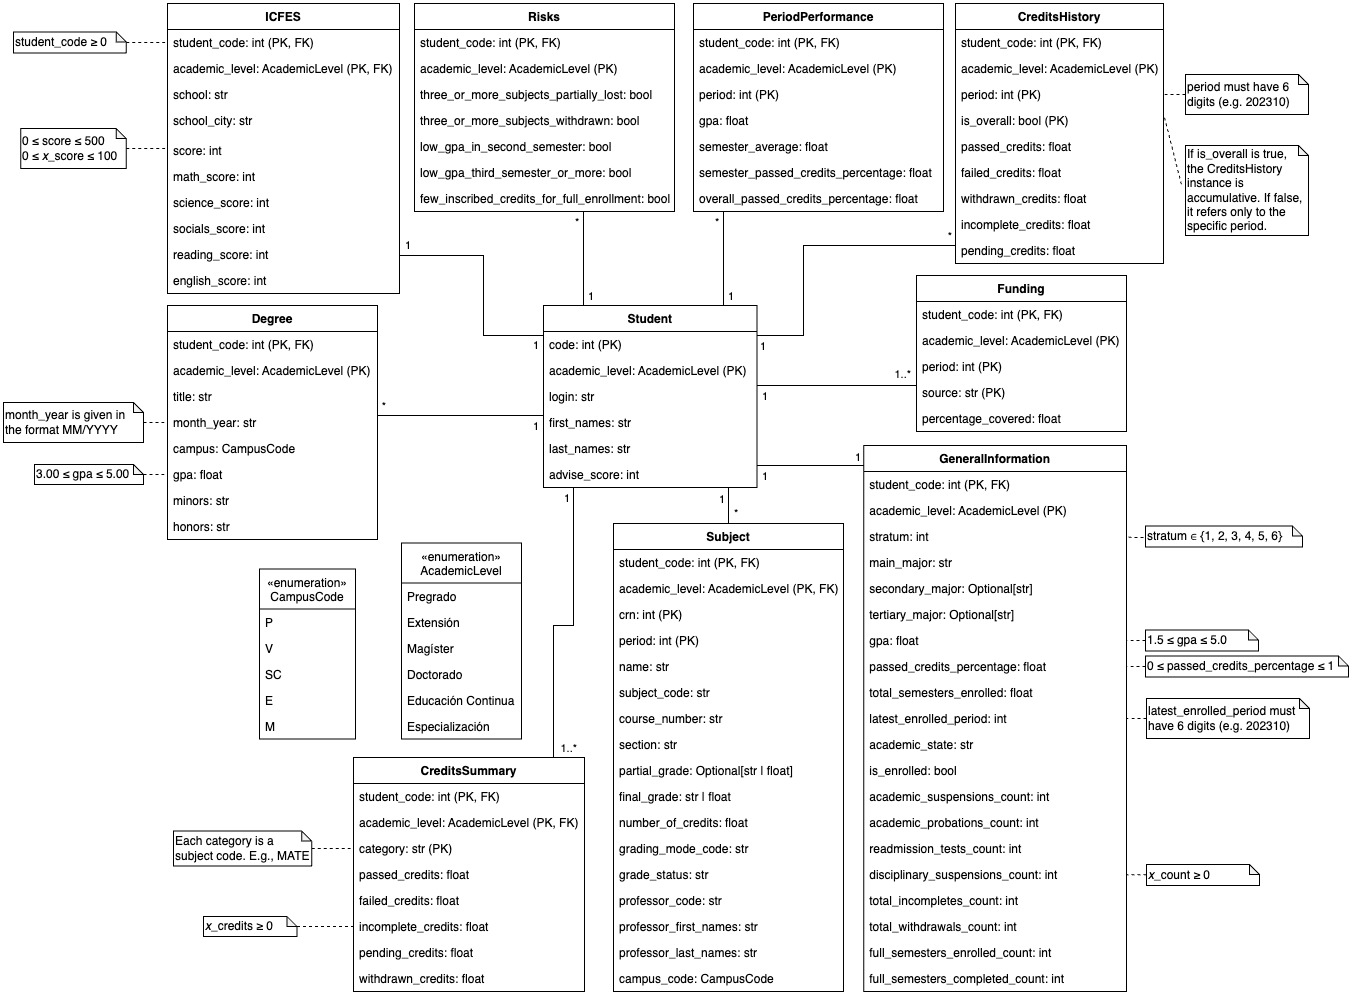
\includegraphics[width=\textwidth]{img/diagrama-clases.jpg}
	\caption{Diagrama de clases del \gls{API}}
	\label{fig:diagrama_clases}
\end{figure}

El diagrama de clases está escrito en inglés, siguiendo las convenciones de \gls{UML}. Cada clase tiene un nombre, que es un sustantivo en singular, y una serie de atributos. Los atributos están escritos en el formato \texttt{nombre: tipo}, donde \texttt{nombre} es el nombre del atributo y \texttt{tipo} es el tipo de dato del atributo. Por conveniencia, los tipos de datos empleados son los mismos que se utilizan en el lenguaje de programación \gls{Python}, que es el lenguaje en el que se implementa el \gls{API}, pero bien podrían usarse los tipos de datos de cualquier otro lenguaje de programación orientado a objetos sin afectar semánticamente el diagrama de clases, por lo que mantiene su independencia de la implementación.

\subsubsection{Clases del API}

La estructura de clases del \gls{API} se basa en el principio de responsabilidad única, que establece que cada clase debe tener una sola responsabilidad y representar un solo concepto en el dominio del problema. Las clases propuestas en el diagrama se presentan alfabetizadas en la tabla \ref{tab:clases}, con su nombre original en inglés, la traducción al español y una breve descripción de su responsabilidad.

\begin{longtblr}[
		caption = {Clases del \gls{API} y sus responsabilidades},
		label = {tab:clases},
	]{
		colspec = {X[1,l] X[1,l] X[2,l]}
	}
	\hline
	\textbf{Nombre original} & \textbf{Nombre traducido}       & \textbf{Responsabilidad}                                                                                                                                                                                                                                                                                             \\
	\hline
	CreditsHistory           & Historial de créditos           & Rastrea el estado global de los créditos del estudiante, incluyendo: aprobados, reprobados, retirados, pendientes e incompletos, tanto para periodos específicos, por ejemplo un semestre particular, como en general y hasta la fecha.                                                                                  \\
	CreditsSummary           & Resumen de créditos             & Proporciona un desglose categórico de los créditos aprobados, reprobados, retirados, pendientes e incompletos, para una categoría específica de materias. Algunos ejemplos de categoría pueden ser: las materias de la carrera principal, las materias de matemáticas, las materias de física, entre otras.          \\
	Degree                   & Título                          & Almacena información sobre los títulos académicos obtenidos por el estudiante, como el nombre del título, el campus, el promedio y menciones especiales, como títulos con honores.                                                                                                                                   \\
	Funding                  & Financiamiento                  & Detalla las fuentes de financiamiento del estudiante, que pueden incluir becas y créditos educativos, con el porcentaje cubierto por cada fuente.                                                                                                                                                                    \\
	GeneralInformation       & Información general             & Contiene datos generales del estudiante, como su carrera principal, estrato, GPA actual, entre otros indicadores relevantes.                                                                                                                                                                                         \\
	ICFES                    & ICFES                           & Almacena los puntajes del estudiante en las áreas evaluadas por el examen ICFES, como matemáticas, lectura y ciencias.                                                                                                                                                                                               \\
	PeriodPerformance        & Rendimiento por\newline periodo & Guarda información del desempeño académico del estudiante en un periodo específico, incluyendo el promedio del semestre y el porcentaje de créditos aprobados.                                                                                                                                                       \\
	Risks                    & Riesgos                         & Identifica indicadores de riesgo académico, como bajo GPA en los primeros semestres o retiro de múltiples materias.                                                                                                                                                                                                  \\
	Student                  & Estudiante                      & Representa a un estudiante de la universidad cuando se encontraba en un nivel académico específico. Almacena la información esencial para la identificación del estudiante, como nombres, apellidos, código y usuario (\texttt{login}, que corresponde al nombre de usuario en el correo electrónico institucional). \\
	Subject                  & Materia                         & Representa una materia específica cursada por el estudiante, incluyendo el nombre, el código, los créditos, el profesor, la nota obtenida y el estado de la materia.                                                                                                                                                 \\
	\hline
\end{longtblr}

Como complemento del diagrama de clases y de la tabla \ref{tab:clases}, vale la pena ahondar en algunas de las decisiones de diseño que se tomaron en la creación de las clases con base en el dominio del negocio:
\begin{itemize}
	\item La clase \texttt{Student} es la clase principal del modelo. Salta a la vista que no representa a un estudiante por completo, sino que representa a un estudiante en un nivel académico específico. Esto se debe a que resulta conveniente tratar de forma distinta al mismo estudiante en diferentes niveles académicos, ya que su contexto puede haber cambiado significativamente: el título al que aspira es distinto, las materias que cursa son distintas, su desempeño académico puede haber mejorado o empeorado, e incluso su situación socioeconómica puede haber cambiado. La misma persona en pregrado no puede ser tratada de la misma forma que en posgrado.
	\item La clase \texttt{CreditsSummary} es una clase auxiliar que se encarga de proporcionar un desglose categórico de los créditos aprobados, reprobados, retirados, pendientes e incompletos, para una categoría específica de materias. Naturalmente, no para todos los estudiantes se incluyen las mismas categorías. Es decir, para un estudiante de ingeniería, Categorías relevantes pueden ser las materias Específicas de su rama del ingeniería, las materias de matemática y las materias de física. Sin embargo, para un estudiante de arte, incluso si el estudiante ha optado por cursar materias de matemática y física, esas categorías pueden no ser relevantes para su desempeño académico. Esto es un matiz que es difícil representar en un diagrama de clases, pues corresponde a especificidades del dominio del problema, por lo cual se aclara en este apartado.
	\item Puede que el lector se haya percatado que la clase \texttt{Risks} está nombrada con un sustantivo en plural, lo cual aparentemente transgrede las convenciones de construcción de diagramas de clase. Eso no es un error, sino una decisión consciente de diseño. Se debe a que la clase \texttt{Risks} no representa un riesgo académico en particular, sino que cada instancia de la clase corresponde a un conjunto de riesgos académicos, entre ellos bajo GPA y retiro de múltiples materias. Por lo tanto, el nombre en plural es más adecuado que el nombre en singular para representar la naturaleza de la clase.
\end{itemize}

\subsubsection{Relaciones entre las clases}

Las relaciones entre las clases se representan mediante líneas que unen las clases. Las relaciones en este diagrama son muy simples, lo cual fue una elección deliberada en pos de la simplicidad y la claridad. Cada línea representa una asociación entre dos clases y en sus extremos cuenta con números que indican la multiplicidad de la asociación, es decir, cuántos objetos de una clase están asociados con cuántos objetos de la otra clase. Un asterisco indica que hay muchos objetos asociados, mientras que un número indica la cantidad exacta de objetos asociados. 

Como ejemplo, considérese la asociación entre la clase \texttt{Student} que representa a un estudiante y la clase \texttt{Degree} que representa un grado. Un estudiante puede estar asociado con algún grado, en caso de ya haberse graduado, con varios, en caso de haber obtenido varios grados, o con ninguno, en caso de no haberse graduado. Sin embargo, cada grado corresponde unívocamente a un estudiante. Por ende, la asociación entre la clase \texttt{Student} y la clase \texttt{Degree} es de uno a muchos, representada por la línea que une ambas clases con un 1 en el extremo de la clase \texttt{Student} y un asterisco en el extremo de la clase \texttt{Degree}.

La tabla \ref{tab:relaciones} detalla las relaciones entre las clases del diagrama de clases, con una breve descripción de la relación y la multiplicidad de la asociación. Se organizan en orden de aparición, de arriba a abajo y de izquierda a derecha, en el diagrama de clases.


\begin{longtblr}[
		caption = {Relaciones entre las clases del diagrama de clases},
		label = {tab:relaciones},
	]{
		colspec = {X[1,l] X[2,l] X[3,l]}
	}

	\hline
	\textbf{Clase 1} & \textbf{Clase 2}            & \textbf{Descripción y Multiplicidad}                                                                                                                         \\  \hline
	\texttt{Student} & \texttt{GeneralInformation} & Un estudiante está asociado con una única instancia de información general. Multiplicidad: 1 a 1.                                                            \\
	\texttt{Student} & \texttt{ICFES}              & Un estudiante puede tener una única instancia de resultados del ICFES. Multiplicidad: 1 a 1.                                                                 \\
	\texttt{Student} & \texttt{Risks}              & Un estudiante tiene una única instancia de indicadores de riesgos académicos. Multiplicidad: 1 a 1.                                                          \\
	\texttt{Student} & \texttt{PeriodPerformance}  & Un estudiante puede estar asociado con muchos periodos de desempeño académico. Multiplicidad: 1 a muchos.                                                    \\
	\texttt{Student} & \texttt{CreditsHistory}     & Un estudiante puede tener muchos historiales de créditos, cada uno relacionado con un periodo específico o de manera acumulativa. Multiplicidad: 1 a muchos. \\
	\texttt{Student} & \texttt{CreditsSummary}     & Un estudiante tiene un resumen de créditos categorizado. Multiplicidad: 1 a 1.                                                                               \\
	\texttt{Student} & \texttt{Subject}            & Un estudiante está asociado con muchas materias, pero cada materia pertenece a un único estudiante. Multiplicidad: 1 a muchos.                               \\
	\texttt{Student} & \texttt{Degrees}            & Un estudiante puede haber obtenido múltiples títulos. Multiplicidad: 1 a muchos.                                                                             \\
	\texttt{Student} & \texttt{Funding}            & Un estudiante puede tener múltiples fuentes de financiamiento. Multiplicidad: 1 a muchos.                                                                    \\
	\texttt{Subject} & \texttt{CreditsSummary}     & Cada materia está categorizada en un resumen de créditos. Multiplicidad: 1 a 1.
	\\
	\hline
\end{longtblr}

\subsubsection{Reglas de negocio en el diagrama de clases}

En el diagrama de clases se pueden evidenciar anotaciones en algunos atributos. Varias de estas anotaciones corresponden a restricciones de integridad que se deben cumplir en el modelo de datos, que en últimas representan reglas del dominio del problema. A esto, usualmente se le denomina \textit{reglas de negocio} y son restricciones que se deben cumplir en el modelo de datos para que reflejen la realidad de manera fiel.

La tabla \ref{tab:anotaciones} detalla las anotaciones en el diagrama de clases que tienen esa función, junto con su significado en términos del dominio del problema, es decir, en el contexto de la Universidad. Se organizan en orden de aparición en el diagrama de clases, de arriba a abajo y de izquierda a derecha.

\begin{longtblr}[
		caption = {Anotaciones del diagrama de clases y su significado},
		label = {tab:anotaciones},
	]{
		colspec = {X[1,l] X[2,l] X[2,l]},
	}
	\hline
	\textbf{Anotación}                                                           & \textbf{Significado}                                                                                                       & \textbf{Justificación}                                                                                                                                                                                                                                             \\
	\hline
	\texttt{student\_code \ensuremath{\geq} 0}                                   & El código del estudiante debe ser mayor o igual a 0                                                                        & El código del estudiante debe ser un entero positivo que identifica únicamente a cada estudiante. No se permiten códigos negativos.                                                                                                                                \\
	\texttt{0 \ensuremath{\leq} score \ensuremath{\leq} 500}                     & El puntaje del ICFES (formalmente, la prueba Saber 11) debe estar entre 0 y 500                                            & El puntaje máximo en la prueba Saber 11 es 500, y el mínimo es 0.                                                                                                                                                                                                  \\
	\texttt{0 \ensuremath{\leq} x\_score \ensuremath{\leq} 100}                  & Los puntajes de las áreas evaluadas por el ICFES deben estar entre 0 y 100                                                 & Los puntajes de las áreas evaluadas por el ICFES se normalizan a una escala de 0 a 100.                                                                                                                                                                            \\
	\texttt{month\_year is given in the format MM/YYYY}                          & La fecha de graduación, que se representa como un mes y un año, debe tener el formato MM/YYYY                              & La fecha de graduación se codifica en el formato de mes y año para garantizar consistencia en los registros.                                                                                                                                                       \\
	\texttt{3.00 \ensuremath{\leq} gpa \ensuremath{\leq} 5.0}                    & El GPA debe estar entre 3.0 y 5.0                                                                                          & En el sistema de la Universidad, el GPA mínimo para graduarse es 3.0 y el máximo posible es 5.0.                                                                                                                                                                  \\
	\texttt{Each category is a subject code. E.g., MATE}                         & Cada categoría de un Resumen de créditos es un código de materia. Por ejemplo, MATE representa las materias de matemáticas & Las categorías de un Resumen de créditos se representan con códigos de materia. Esta decisión de diseño se explica en detalle arriba, en la descripción de la clase \texttt{CreditsSummary}.                                                                       \\
	\texttt{x\_credits \ensuremath{\geq} 0}                                      & Los créditos aprobados, reprobados, retirados, pendientes e incompletos deben ser mayores o iguales a 0                    & No tiene sentido registrar un número negativo de créditos en ningún contexto académico.                                                                                                                                                                            \\
	\texttt{period must have 6 digits (e.g. 202310)}                             & El periodo académico debe tener 6 dígitos                                                                                  & Los periodos académicos se codifican en el formato de año seguido por el indicador del tipo de periodo. Usualmente se usa un guión entre el año y el tipo de periodo, e.g., 2023-10, pero en este caso resulta más conveniente usar un número entero de 6 dígitos. \\
	\texttt{stratum \ensuremath{\in} \{1, 2, 3, 4, 5, 6\}}                       & El estrato socioeconómico debe estar entre 1 y 6                                                                           & Los estratos socioeconómicos en Colombia están normados en este rango por ley. Si el estudiante no reside en Colombia, no se registra su estrato.                                                                                                            \\
	\texttt{1.5 \ensuremath{\leq} gpa \ensuremath{\leq} 5.0}                     & El GPA debe estar entre 1.5 y 5.0                                                                                          & En el sistema de la Universidad, el GPA mínimo posible es 1.5, y el máximo posible es 5.0.                                                                                                                                                                         \\
	\texttt{0 \ensuremath{\leq} passed\_credits\_percentage \ensuremath{\leq} 1} & El porcentaje de créditos aprobados debe estar entre 0 y 1                                                                 & Todo porcentaje es un número entre 0 y 1, inclusive.                                                                                                                                                                                                               \\
	\texttt{latest\_enrolled\_period must have 6 digits (e.g. 202310)}           & El periodo académico más reciente en el que el estudiante estuvo inscrito debe tener 6 dígitos                             & Esta explicación es análoga a la de la anotación \texttt{period must have 6 digits (e.g. 202310)}.                                                                                                                                                                 \\
	\hline
\end{longtblr}

\section{Implementación del API}

Esta sección se ocupa de la implementación del \gls{API REST}. En particular, se centra en los aspectos técnicos relacionados con el desarrollo del \gls{API}, incluyendo el lenguaje de programación, el framework y las herramientas asociadas a la implementación.

\subsection{Lenguaje y framework}

El \gls{API REST} está implementado en \gls{Python}, utilizando el framework \gls{FastAPI}. Se dedica un apartado a justificar la elección de cada uno de ellos.

\subsubsection{Python}

Un breve pero excelente resumen de las características del lenguaje se encuentra en la documentación oficial:
\begin{quote}
	\gls{Python} es un lenguaje interpretado, interactivo y orientado a objetos. Incorpora módulos, excepciones, tipado dinámico, tipos de datos dinámicos de muy alto nivel y clases. Además de la programación orientada a objetos, admite múltiples paradigmas de programación, como la programación procedural y funcional. \gls{Python} combina una potencia notable con una sintaxis muy clara. Ofrece interfaces a numerosas llamadas y bibliotecas del sistema, así como a distintos sistemas de ventanas, y es extensible en C o C++. También puede utilizarse como lenguaje de extensión para aplicaciones que requieran una interfaz programable. Finalmente, \gls{Python} es portátil: se ejecuta en diversas variantes de Unix, incluyendo Linux y macOS, así como en Windows. \cite{python_official_docs}
\end{quote} % TODO: Solve extra spacing issue
\noindent Existe una infinidad de argumentos técnicos para usar \gls{Python} en cualquier proyecto de software, que están bien documentadas en muchísimos recursos; por ejemplo, \cite{learning_python} tiene en su primer capítulo una sección dedicada exclusivamente a las razones por las cuales millones de desarrolladores alrededor del mundo usan el lenguaje. Por ende, no ahondaré en razones técnicas para elegir \gls{Python}.

No obstante, cabe mencionar una que existe una justificación contextual para elegir \gls{Python} para la implementación del \gls{API REST}, la cual es independiente de sus virtudes técnicas y responde a preocupaciones por la mantenibilidad del proyecto. En concreto, \gls{Python} es el principal lenguaje de programación que se enseña en la Universidad. Bajo la estructura curricular actual, en todos los programas de las facultades de Ingeniería, Ciencias y Economía, el curso ISIS-2021: Introducción a la Programación es obligatorio y constituye el primer curso de programación. % TODO: Cita!

Este curso, que \say{introduce conceptos básicos de programación, utilizados para resolver problemas con un programa de computadora} \cite{ip}, se enseña enteramente en \gls{Python}. El siguiente curso de programación, ISIS-1225: Estructuras de Datos y Algoritmos, que es obligatorio para los programas de Matemática e Ingeniería de Sistemas y Computación, también se enseña en \gls{Python}. % TODO: Cita!
Por lo tanto, la mayoría de los estudiantes de la Universidad que cursan programas del área de STEM tienen experiencia previa en \gls{Python} y varios no tienen experiencia en ningún otro lenguaje de programación. Esta restricción contextual implicó que la elección de \gls{Python} para la implementación del \gls{API REST} fue prácticamente obligatoria en aras de garantizar la sostenibilidad del proyecto a largo plazo.

\subsubsection{FastAPI}

\say{\gls{FastAPI} es un framework moderno, rápido (de alto rendimiento) y fácil de usar para construir \glslink{API}{APIs} con \gls{Python} basado en las anotaciones de tipo estándar de \gls{Python}} \cite{fastapi_docs}.

La principal justificación para la elección de \gls{FastAPI} va de la mano con la alta prioridad que se le ha dado a la mantenibilidad del proyecto. Se buscaba un framework que tuviera una curva de aprendizaje corta para desarrolladores familiarizados con \gls{Python}, que fuera fácil de mantener y extender, y que facilitara construir buena documentación. Sorprendentemente, \gls{FastAPI} cumple con todos estos requisitos, sin comprometer su rendimiento. De hecho, \gls{FastAPI} es uno de los frameworks más rápidos para construir \glslink{API}{APIs} con \gls{Python}, superando a otros frameworks populares como Flask y Django \cite{fastapi_benchmarks}.

Respecto a la facilidad de aprendizaje, la sintaxis \gls{FastAPI} está basada en las anotaciones de tipo estándar de \gls{Python}. Esto permite que para cualquier desarrollador que conozca \gls{Python}, sea sencillo aprender \gls{FastAPI}, pues no requiere aprender sintaxis adicional. \cite{fastapi_features}. Respecto a la mantenibilidad del framework, se destaca su integración con herramientas de validación de datos, como \gls{Pydantic}, que permite definir modelos de datos y validar automáticamente los datos entrantes. Esta funcionalidad facilita el mantenimiento del código en tanto que cualquier cambio en los modelos de datos se refleja inmediatamente en la validación de los datos entrantes \cite{fastapi_features}.

Por último, se destaca la integración con herramientas de documentación automática. \gls{FastAPI} genera automáticamente documentación interactiva de la \gls{API REST}, que se puede acceder a través de dos rutas: \verb|/docs| y \verb|/redoc|. La primera ruta genera una interfaz interactiva basada en \gls{Swagger}, mientras que la segunda ruta genera una interfaz interactiva basada en \gls{Redoc} \cite{fastapi_features}. Ambas interfaces permiten explorar los recursos del \gls{API REST}, probarlos y ver la documentación generada automáticamente, lo cual simplifica enormemente la tarea de mantener el \gls{API REST}, ya que cualquier cambio en el código se ve reflejado en la documentación.

Las razones anteriores hacen de \gls{FastAPI} una excelente elección para la implementación de cualquier \gls{API}, y más para este proyecto en particular, considerando las restricciones contextuales enunciadas en la sección anterior.

\subsection{Estructura de directorios}

\gls{FastAPI} es un framework no opinionado, es decir, que permite al desarrollador elegir cómo estructurar su proyecto. Esto significa que hay una infinidad de formas de estructurar un proyecto de \gls{FastAPI}. La siguiente fue la estructura de directorios elegida para este proyecto:
\begin{itemize}
	\item \texttt{README.md}
	\item \texttt{app.log}
	\item \texttt{db/}
	\item \texttt{.env}
	\item \texttt{dev.log}
	\item \texttt{requirements.txt}
	\item \texttt{sonar-project.properties}
	\item \texttt{src/}
	\begin{itemize}
			\item \texttt{\_\_init\_\_.py}
			\item \texttt{main.py}
			\item \texttt{authentication/}
			\item \texttt{azure\_interface/}
			\item \texttt{config/}
			\item \texttt{constants/}
			\item \texttt{files/}
			\item \texttt{models/}
			\item \texttt{persist\_from\_blobs/}
			\item \texttt{routers/}
			\item \texttt{schemas/}
			\item \texttt{services/}
			\item \texttt{utils/}
	\end{itemize}
	\item \texttt{tests/}
\end{itemize}

Nótese que no se reflejan todos los archivos y directorios del proyecto, sino únicamente aquellos que son relevantes para la estructura de código del \gls{API REST}. La tabla \ref{tab:estructura_directorios} detalla la función de cada directorio y archivo en el directorio raíz del proyecto.

\begin{longtblr}[
		caption = {Estructura de archivos y directorios del proyecto},
		label = {tab:estructura_directorios},
	]{
		colspec = {X[1,l] X[3,l]},
	}
	\hline
	\textbf{Directorio/Archivo} & \textbf{Descripción}
	\\
	\hline
	\texttt{README.md} & Archivo con documentación fundamental del proyecto, en concreto una breve descripción e instrucciones de ejecución del proyecto en un ambiente local. Está escrito en \gls{Markdown}, que es un lenguaje de marcado ligero, es decir, que permite dar formato al texto de forma sencilla. \\
	\texttt{app.log} & Archivo de registro (\textit{log}) generado automáticamente en el que se almacena información como errores, advertencias y notificaciones generadas durante la ejecución de la aplicación. El archivo \texttt{app.log} corresponde al entorno de producción; en el entorno de desarrollo se genera el archivo \texttt{dev.log}, cuyo propósito es análogo. Se ahonda en el uso de este archivo en la sección \ref{sec:despliegue_api} \\
	\texttt{db/} & Directorio que almacena scripts relacionados con respaldos y restauración de la base de datos, además de otros archivos necesarios para la gestión de datos persistentes. \\
	\texttt{.env} & Archivo de configuración que almacena variables de entorno. Estas variables permiten definir valores sensibles o específicos del entorno, como: credenciales, configuraciones de la base de datos, claves o modos de ejecución (desarrollo, pruebas y producción), sin incluirlos directamente en el código fuente. El archivo no se incluye en el control de versiones por contener información sensible, pero en el README se incluyen instrucciones para construirlo, mientras se cuente con las credenciales necesarias. \\
	\texttt{sonar-project}\newline\texttt{.properties} & Archivo de configuración para \gls{SonarQube}. El uso del archivo y de \gls{SonarQube} se explica en la sección \ref{sec:calidad_codigo}. \\
	\texttt{src/} & Directorio principal que contiene el código fuente del proyecto. Su nombre es una abreviación convencional para \textit{source}, que en inglés significa \textit{fuente}. \\
	\texttt{tests/} & Directorio que contiene las \gls{pruebas unitarias} del proyecto. Se ahonda en las \gls{pruebas unitarias} en la sección \ref{sec:calidad_codigo}. \\
	\hline
\end{longtblr}

Como complemento a la tabla \ref{tab:estructura_directorios}, la tabla \ref{tab:estructura_directorios_src} especifica la función de cada directorio y archivo dentro del directorio \texttt{src/}.

\begin{longtblr}[
	caption = {Estructura de archivos y directorios dentro de \texttt{src/}},
	label = {tab:estructura_directorios_src},
]{
	colspec = {X[1,l] X[3,l]},
}
\hline
\textbf{Directorio/Archivo} & \textbf{Descripción}
\\
\hline
	\texttt{\_\_init\_\_.py} & Archivo vacío cuyo nombre indica que el directorio es un paquete en \gls{Python}. \\
	\texttt{main.py} & Punto de entrada de la aplicación. Contiene la configuración del objeto \texttt{\gls{FastAPI}}, que es la instancia principal de la aplicación, la importación e inicialización de las rutas y la configuración de los \textit{\glslink{middleware}{middlewares}}. \\
	\texttt{authentication/} & Módulo que gestiona la autenticación y autorización de usuarios en el proyecto. \\
	\texttt{azure\_interface/} & Módulo que contiene la lógica para interactuar con servicios de Azure. \\
	\texttt{config/} & Módulo que almacena configuraciones del proyecto y de su interacción con la base de datos. \\
	\texttt{constants/} & Módulo que define constantes compartidas utilizadas en el proyecto. \\
	\texttt{files/} & Directorio que almacena archivos estáticos o temporales necesarios para el proyecto. \\
	\texttt{models/} & Módulo en el que se definen las clases que representan las tablas de la base de datos, apalancándose de \gls{SQLAlchemy}, que actúa como \gls{ORM}. \\
	\texttt{persist\_from\_blobs/} & Módulo encargado de la persistencia de datos provenientes de \gls{BLOB}s o almacenamiento de objetos. \\
	\texttt{routers/} & Módulo que define las rutas del \gls{API REST}, organizando los puntos de entrada según su funcionalidad. \\
	\texttt{schemas/} & Módulo que define los esquemas de datos utilizados en el \gls{API REST}, como las estructuras para solicitudes y respuestas.\\
	\texttt{services/} & Módulo que implementa las operaciones que es posible realizar sobre los recursos del API con base en la lógica de negocio del proyecto. \\
	\texttt{utils/} & Módulo que agrupa funciones auxiliares utilizadas en diferentes partes del proyecto.\\
\hline
\end{longtblr}

Vale la pena ahondar en cuatro de los directorios mencionados arriba, que constituyen el esqueleto de cualquier \gls{API}: \texttt{models}, que representa el modelo de datos del \gls{API}; \texttt{schemas}, que define los esquemas de datos utilizados en las solicitudes y respuestas del \gls{API}; \texttt{services}, que contiene la lógica de negocio del proyecto; y \texttt{routers}, que define las rutas del \gls{API REST}. Se dedica un apartado a cada uno de ellos.

\subsubsection{Modelos de datos}

El módulo \texttt{models} contiene las clases que representan las tablas de la base de datos. En particular, cada archivo de \gls{Python} en el directorio \texttt{models} define una clase que abstrae la estructura de una de las tablas de la base de datos relacional. La mayoría de los atributos de la clase corresponden a las columnas de la tabla y algunos atributos especiales definen las relaciones entre las tablas y las restricciones de integridad. Por ejemplo, la clase \texttt{Student} en el archivo \texttt{models/student.py} plasma la tabla \texttt{students} en la base de datos.

Esta abstracción, en la que el modelo de datos relacional se expresa como un modelo de objetos, es una tarea común en el desarrollo de software en lenguajes orientados a objetos y convencionalmente se realiza siguiendo el patrón \gls{ORM} (\textit{Object-Relational Mapper}). Dicho patrón permite representar objetos como tablas en una base de datos relacional y viceversa, a pesar de la diferencia en las estructuras orientada a objetos y relacional (problema conocido como \textit{impedancia de mapeo}, en inglés \textit{object-relational impedance mismatch}). En este proyecto, la librería \gls{SQLAlchemy} encapsula la lógica de mapeo objeto-relacional, permitiendo que las clases de \gls{Python} se mapeen directamente a tablas de la base de datos relacional. El lector puede ser familiar con otros \glslink{ORM}{ORMs}, como JPA (\textit{Java Persistence API}) en Java o \textit{Entity Framework} en C\#, que cumplen una función análoga.

\subsubsection{Esquemas de datos}
\label{subsec:schemas}

El módulo \texttt{schemas} define las clases que corresponden a los esquemas de datos utilizados en las solicitudes y respuestas del \gls{API}. Estas clases están implementadas utilizando \gls{Pydantic}, una librería que provee validación de datos y la generación automática de documentación para los modelos. Todas las clases relacionadas a una entidad específica se definen en un solo archivo, de manera que en el archivo \texttt{schemas/student.py} se definen las clases que representan los esquemas de datos de la entidad \texttt{Student}.

En general, los esquemas de datos son una abstracción que permite definir la estructura de los datos que se envían y reciben en el \gls{API}, y que facilita la validación de los datos y la generación de documentación. Para lectores familiarizados con otros lenguajes o frameworks de desarrollo web, esta capa del \gls{API} es análoga a los \textit{serializers} de Django en \gls{Python}, los DTOs (\texttt{Data Transfer Objects}) de Spring en Java, las clases de contratos en ASP.NET en C\# y las interfaces o tipos definidos en NestJS en TypeScript, por mencionar algunos ejemplos.

Cada esquema se compone de múltiples clases, cada una de las cuales refleja el propósito de la operación para la que se utiliza. Se escriben cinco clases, cada una con un sufijo que indica su propósito: la clase base (con sufijo \texttt{Base}, de forma que para una entidad \texttt{Entity} la clase base se llamaría \texttt{EntityBase}), cuyo propósito es declarar todos los atributos comunes a todas las clases en pos de minimizar la duplicación de código; la clase para creación de datos (\texttt{EntityCreate}), que consta de los atributos necesarios para crear un objeto; la clase para actualización de datos (\texttt{EntityUpdate}), que contiene los atributos necesarios para actualizar un objeto; y la clase para lectura de datos (\texttt{EntityResponse}), que consta de los atributos mínimos que se devuelven en la respuesta del \gls{API}. Algunos objetos tienen además otra clase de respuesta extendida, con prefijo \texttt{ExtendedResponse}, que contiene atributos adicionales que no son necesarios en todas las respuestas, pero que pueden ser útiles en ciertos contextos. Cada clase contiene configuraciones adicionales que proporcionan ejemplos representativos de los datos, que se ven reflejados automáticamente en la documentación del \gls{API}.

Esta estructura modular y estándar para todos los esquemas de datos facilita la reutilización del código y mantiene la consistencia dentro del proyecto. Incluso si los atributos necesarios para crear una clase y los necesarios para actualizarla son los mismos, se definen en clases separadas para mantener la coherencia y facilitar la extensión en el futuro. Al mantener una separación tan definida entre las estructuras de datos utilizadas en las peticiones y respuestas del \gls{API}, y las utilizadas internamente (como los modelos de la base de datos), se facilita el mantenimiento del proyecto, se evitan dependencias innecesarias y se reduce el riesgo de \gls{sobreexposición}, es decir, de entregar más información de la necesaria en las respuestas del \gls{API}. Eso último es especialmente importante en un proyecto que maneja datos sensibles, como el presente.

\subsubsection{Lógica de negocio}

El módulo \texttt{services} contiene las funciones que implementan la lógica de negocio del proyecto. Cada archivo en este módulo encapsula todas las operaciones relacionadas con una clase específica. Por ejemplo, el archivo \texttt{services/student.py} contiene todas las operaciones que se pueden realizar sobre la entidad \texttt{Student}.

Al interior de cada servicio existen, como mínimo, las funciones necesarias para realizar todas las operaciones \gls{CRUD} (crear, leer, actualizar y eliminar, del inglés \textit{Create, Read, Update, Delete}) sobre la entidad correspondiente, y en algunos casos, funciones adicionales que implementan operaciones más complejas. Cada operación se organiza claramente y se nombra con un prefijo que indica su responsabilidad: las funciones para creación (prefijadas con \texttt{create}, de manera que para una entidad \texttt{Entity} la función se llamaría \texttt{create\_entity}) reciben datos validados y los almacenan en la base de datos; las funciones para lectura (\texttt{get\_entity\_by\_id}, \texttt{get\_all\_entities}) realizan consultas específicas o generales sobre los modelos; las funciones para actualización (\texttt{update\_entity}) modifican registros existentes; y las funciones para eliminación (\texttt{delete\_entity}) eliminan los registros de la base de datos de manera controlada. Esta estructura estándar asegura que las operaciones básicas son consistentes en todas las entidades.

En cada función, el servicio interactúa tanto con los modelos como con los esquemas de datos. Los esquemas de datos se utilizan para validar los argumentos que cada función recibe. Se mencionó en la subsección \ref{subsec:schemas} que en cada esquema de datos se definen clases para creación (\texttt{Create}) y actualización (\texttt{Update}); estas clases se utilizan para validar los datos que ingresan a las funciones de creación (\texttt{create\_entity}) y actualización (\texttt{update\_entity}) de los servicios, respectivamente. Por su parte, los modelos cumplen su función como abstracción de la base de datos ofreciendo una interfaz orientada a objetos para interactuar con las tablas, permitiendo que cada función realice las operaciones correspondientes sobre los registros de la base de datos. Por ejemplo, la función \texttt{create\_student}, cuya responsabilidad es crear un estudiante, recibe un objeto de tipo \texttt{CreateStudent}, cuya estructura es validada automáticamente por \gls{Pydantic}, y lo utiliza para crear una instancia del modelo \texttt{Student}, que representa una nueva entrada en la tabla de estudiantes de la base de datos.

Durante el proceso de ejecutar la operación que le corresponde, cada función del servicio se encarga de verificar las reglas de negocio asociadas que son demasiado intricadas como para ser validadas por \gls{Pydantic}. Verbigracia, \gls{Pydantic} puede validar fácilmente que el periodo académico ingresado sea un número, pero no puede verificar que el periodo académico sea válido en el contexto de la Universidad; esta verificación corresponde a la lógica de negocio y se realiza en la función del servicio correspondiente. Varios ejemplos de estas reglas de negocio se mencionan en la tabla \ref{tab:anotaciones}.

En términos de analogía con otras tecnologías, el módulo \texttt{services} es equivalente a las capas de servicio (\textit{service layers}) en frameworks como Spring en Java, los servicios en ASP.NET en C\#, y las clases de servicios en NestJS en TypeScript. Todos estos enfoques tienen como objetivo separar la lógica de negocio tanto de los objetos que representan los datos como de las rutas del API y las representaciones de los recursos.

\subsubsection{Rutas del API}
% TODO: Pedazos de código rebasan el margen
El módulo \texttt{routers} define las rutas del \gls{API REST}, sirviendo como punto de entrada para las solicitudes \gls{HTTP} realizadas al sistema. Cada archivo en este módulo agrupa las rutas relacionadas con una entidad específica. Por ejemplo, el archivo \texttt{routers/student.py} define las rutas bajo el prefijo \texttt{/students}, donde cada ruta corresponde a una operación específica relacionada con la entidad \texttt{Student}.

Cada ruta está asociada a una operación del \gls{API} cuya lógica está implementada en los servicios. Por ende, dependiendo del contenido del servicio, una ruta puede corresponder a una operación básica \gls{CRUD} o una operación personalizada que satisface necesidades específicas del negocio. Cada ruta está implementada como una función dentro del archivo y está decorada con un decorador de \gls{FastAPI} que indica el método \gls{HTTP} correspondiente. Los decoradores disponibles son \texttt{@router.get}, \texttt{@router.post}, \texttt{@router.put} y \texttt{@router.delete}, correspondientes a las operaciones estándar de \gls{HTTP}: \texttt{GET}, \texttt{POST}, \texttt{PUT} y \texttt{DELETE}. 

Un aspecto clave del diseño es la interacción entre las rutas, los servicios (\texttt{services}) y los esquemas (\texttt{schemas}). Las funciones de los \textit{routers} actúan como intermediarias: reciben las solicitudes \gls{HTTP}, validan los datos de entrada utilizando esquemas (\texttt{schemas}), delegan la lógica de negocio a las funciones correspondientes en los servicios y entregan respuestas estructuradas basadas en los esquemas de datos. Por ejemplo, una función que crea un estudiante utilizará un esquema \texttt{StudentCreate} para validar los datos de entrada, invocará a la función \texttt{create\_student} del servicio que encapsula la creación del estudiante y entregará una respuesta estructurada utilizando el esquema \texttt{StudentResponse} (o \texttt{StudentExtendedResponse} si la ruta en cuestión requiere información adicional).

A causa del flujo anterior, los esquemas de tipo \texttt{Response}, como \texttt{StudentResponse}, desempeñan un papel fundamental en este proceso. Estos esquemas aseguran que las respuestas del \gls{API} estén estructuradas de manera consistente, incluyendo únicamente los atributos necesarios para el cliente y excluyendo información interna o sensible. 

Además de las operaciones \gls{CRUD}, los \textit{routers} incluyen validaciones adicionales para garantizar que las solicitudes sean válidas antes de delegar el procesamiento a los servicios. Estas validaciones pueden incluir la verificación de que los identificadores no sean nulos, que los datos ingresados sean válidos y que los recursos existan antes de realizar operaciones sobre ellos. Por ejemplo, una solicitud para eliminar un estudiante puede comprobar primero si el estudiante existe, averiguándolo a través del servicio, antes de llamar a la función de eliminación del servicio.

En términos de arquitectura, el módulo \texttt{routers} es análogo a los controladores (\textit{controllers}) en frameworks como Spring en Java, ASP.NET en C\#, o NestJS en TypeScript. Al igual que en estas tecnologías, el propósito de los \textit{routers} es mantener la independencia entre la lógica de negocio y la lógica de la interfaz de usuario, de forma que los cambios en la lógica de negocio no afecten la interfaz de usuario y viceversa.

\section{Calidad de código}
\label{sec:calidad_codigo}

Teniendo en cuenta que el software producido es de alto valor para la universidad y, por ende, probablemente deberá ser mantenido, extendido y reutilizado en el futuro, su desarrollo fue sometido a rigurosos estándares de calidad de código. Esta sección detalla las herramientas y prácticas empleadas para garantizar la calidad del código.

\subsection{Análisis estático}

El código fuente del \gls{API} está escrito para que sea fácil de entender y mantener.

Se configuró \gls{SonarQube} para realizar análisis estático sobre el código, utilizando el \gls{perfil de calidad} estándar para \gls{Python} 3.11. Esta herramienta identifica posibles problemas en el código y genera métricas detalladas para el monitoreo continuo de la calidad. En particular, la herramienta se cerciora de que el código cumple con estándares mínimos de mantenibilidad, confiabilidad y seguridad.

En este caso, los resultados más recientes del análisis de \gls{SonarQube} se muestran en la figura \ref{fig:sonarqube}.

% TODO: Insertar imagen de SonarQube e interpretación

Más aún, en favor de garantizar un estilo de código uniforme y limpio, se emplearon las siguientes herramientas:
\begin{itemize}
	\item \gls{isort} y \gls{black} como \glslink{formateador}{formateadores} de código. El primero se encarga de ordenar las importaciones de los módulos de \gls{Python} de manera consistente, mientras que el segundo reformatea el código para asegurar un formato consistente. \glslink{black}{Black} garantiza que todos los proyectos de \gls{Python} que lo usan tengan el mismo estilo de código, lo que facilita la lectura y el mantenimiento del código a desarrolladores nuevos.
	\item \gls{Flake8} y \gls{SonarLint} como \glslink{linter}{linters}, para verificar la adherencia a las mejores prácticas y estándares de calidad de código. \gls{Flake8} es una herramienta de verificación de código que busca errores en el estilo del código \gls{Python}, mientras que \gls{SonarLint} es un \gls{linter} que se integra con \gls{SonarQube} y proporciona análisis en tiempo real del código.
\end{itemize}

\subsection{Documentación}

Existe extensa documentación del proyecto, tanto específica del API como general, incluyendo este documento. La documentación del \gls{API} se genera automáticamente a partir de los \glslink{docstring}{docstrings} de las funciones y métodos, gracias a las funcionalidades nativas de \gls{FastAPI} mencionadas arriba, y se puede acceder a través de las rutas \verb|/docs| y \verb|/redoc|.

Para que la documentación generada automáticamente resulte genuinamente útil, es indispensable que los parámetros usados por las funciones estén semánticamente bien nombrados, que los tipos de datos sean explícitos y que todas las funciones estén debidamente documentadas. Para garantizar que ese sea el caso, se emplearon las prácticas descritas a continuación.

En primer lugar, para asegurar que los parámetros de las funciones estén bien nombrados y que los tipos de datos sean explícitos, resulta útil el uso de \gls{Pydantic} en la definición de los esquemas de datos. \gls{Pydantic} permite definir los tipos de datos de los atributos de las clases y automáticamente valida los datos que se le pasan a la clase. Por ejemplo, si se define una clase \texttt{StudentCreate} con un atributo \texttt{name} de tipo \texttt{str}, \gls{Pydantic} se encargará de validar que el valor de \texttt{name} sea una cadena de texto. Esto garantiza que los datos que se pasan a las funciones del \gls{API} sean válidos y que los desarrolladores que utilicen el \gls{API} sepan qué tipo de datos esperar.

En segundo lugar, respecto a la documentación de las funciones y métodos al interior del código, todas las funciones y métodos del \gls{API} están documentados mediante \glslink{docstring}{\textit{docstrings}}, siguiendo las convenciones definidas en el estándar \href{https://peps.python.org/pep-0257/}{\gls{PEP} 257}. Debido a que estas disposiciones son notablemente flexibles, se optó por la convención de \glslink{docstring}{docstrings} de \gls{NumPy}. Más específicamente, se satisfacen todos los lineamientos de la \href{https://python-sprints.github.io/pandas/guide/pandas_docstring.html}{guía de \glslink{docstring}{docstrings} de \gls{Pandas}}. 

Para evitar omisiones, se emplea la librería \verb|flake8-docstrings| para verificar que los \glslink{docstring}{docstrings} sigan la convención de \gls{NumPy}. Esto se configura mediante la opción \verb|docstring-convention=numpy| en el archivo de configuración de \gls{Flake8}.

\subsection{Pruebas y automatización}

Sumado a lo anterior, se integraron diversas herramientas de automatización y pruebas para garantizar la calidad del código en cada modificación. En particular, se destacan las siguientes prácticas:

\begin{itemize}
    \item Se hizo uso de \gls{Pytest} para la creación y ejecución de \gls{pruebas unitarias}. \gls{Pytest} es una librería de pruebas que facilita la escritura y ejecución de pruebas en \gls{Python}. Se eligió \gls{Pytest} por su simplicidad y flexibilidad, que permiten escribir pruebas de manera clara y concisa.
    \item Se implementó un \gls{hook} de pre-commit de \gls{Git}, configurado para garantizar que el código está formateado y probado antes de cada \textit{commit}. El \gls{hook} de pre-commit se encarga de ejecutar \gls{isort}, \gls{black}, \gls{Flake8} y \gls{Pytest} antes de permitir que se realice un \textit{commit}. Si alguna de estas herramientas reporta un error, el \textit{commit} es rechazado y se notifica al desarrollador.
    \item Se dispone de un \gls{pipeline} en \gls{GitHub Actions} que ejecuta las pruebas, genera un reporte de cobertura y lo envía a \gls{SonarQube}. El \gls{pipeline} se ejecuta automáticamente cada vez que se realiza un \textit{push} a la rama principal del repositorio. Si alguna de las pruebas falla, el \gls{pipeline} se detiene y se notifica al desarrollador.
\end{itemize}

Esto garantiza que el código que se envía a producción esté formateado correctamente, sea legible, esté probado y cumpla con los estándares de calidad definidos.

\section{Infraestructura}

Esta sección describe la infraestructura utilizada para el despliegue del \gls{API} y la base de datos. La descripción se realiza a alto nivel y sin entrar en las características de la infraestructura, ya que estas son específicas de la Universidad y no son relevantes para el desarrollo del \gls{API}. Se hace hincapié en la elección de \gls{Docker} como tecnología de contenedores y en la separación de la base de datos en una máquina virtual aparte, por cuestiones de seguridad.

\subsection{Despliegue del API}
\label{sec:despliegue_api}

El despliegue del \gls{API} se realiza mediante el uso de contenedores \gls{Docker}, que permiten garantizar un entorno de ejecución uniforme y reproducible. Estos contenedores se alojan en una máquina virtual proporcionada por la universidad, la cual actúa como servidor central y asegura que el \gls{API} esté disponible de manera continua. La configuración del servidor garantiza que el contenedor de \gls{Docker} se mantenga siempre en ejecución, asegurando así la disponibilidad y la estabilidad del servicio.

El uso de \gls{Docker} ofrece múltiples beneficios. En primer lugar, permite simplificar el proceso de despliegue al encapsular todas las dependencias y configuraciones necesarias en el contenedor. Esto asegura que el \gls{API} se comporte de manera consistente en cualquier entorno, eliminando problemas derivados de diferencias en sistemas operativos o configuraciones locales. Además, facilita significativamente las actualizaciones y el mantenimiento. Cuando se realizan cambios en el \gls{API}, basta con hacer un \textit{pull} del repositorio en la máquina virtual y reiniciar el contenedor para que los cambios sean efectivos. Este enfoque reduce tiempos de inactividad y minimiza errores humanos durante el proceso de despliegue. De hecho, se realizaron pruebas de modificación y despliegue y se determinó que el tiempo de indisponibilidad del servicio tras una actualización es inferior a 5 minutos.

\subsection{Base de datos}

La base de datos utilizada es \gls{PostgreSQL}, una solución robusta, escalable y ampliamente reconocida. \gls{PostgreSQL} ofrece características avanzadas como soporte para transacciones ACID, manejo eficiente de consultas complejas y extensibilidad mediante módulos adicionales. Sumado a eso, es predominantemente la tecnología de bases de datos que se enseña en la Universidad, por lo cual se consideró una elección natural, pensando en la continuidad del proyecto.

Por razones de seguridad, la base de datos \gls{PostgreSQL} reside en una máquina virtual separada, accesible únicamente a través de la red interna Séneca de la universidad. Este diseño implementa una práctica conocida como \textit{air-gapping}, la cual consiste en aislar físicamente o lógicamente un sistema del acceso directo desde redes externas. En este caso, el \textit{air-gapping} asegura que la base de datos no pueda ser accedida desde dispositivos o redes externas a la Universidad, incluso si se dispone de las credenciales.

El uso del \textit{air-gapping} tiene particular sentido en este contexto, considerando la sensibilidad de la información gestionada. Los datos académicos y socioeconómicos del estudiantado están además protegidos por normativas de privacidad y protección de datos, lo cual propulsó la implementación de esta arquitectura.
